\documentclass[11pt,titlepage]{article}
\usepackage[parfill]{parskip}
\usepackage{textcomp}
\usepackage{fullpage}
\usepackage{amsmath}
\usepackage{amssymb}
\usepackage{gensymb}
\usepackage{color}
\usepackage{graphicx}
\graphicspath{ {images/} }
\usepackage{float}
\restylefloat{table}
\usepackage{array}

\author{Rane Brown \\ Brian Douglass}
\title{ECEN 4593: Memory Simulation Project}
\date{\today}

\begin{document}
\maketitle
\tableofcontents
\listoffigures
\listoftables
\newpage

\section{Introduction}
    This project simulates a two level cache using the C programming language. The memory hierarchy consists of a L1 instruction cache, a L1 data cache and a unified L2 cache. In addition, each cache level has an associated victim cache which is setup as an eight deep fully associative cache. If there is a miss at a particular cache level then that level's victim cache is checked before making a request to the next level in the hierarchy. The caches are \emph{write-allocate}, \emph{write-back} caches which means a dirty bit must be used to track when a write request occurs. Each cache maintains a LRU (least recently used) replacement policy for each set in a set associative cache or in a fully associative cache. This project evaluates the performance of nine different memory configurations using sample traces from a selection of six SPEC benchmarks. The bus widths, transfer times, hit/miss times, and various other important parameters can be found in the official project description.

\section{Setup and Code Structure}
    When a simulation is executed, the cache first needs to be structured and built. The structure of the cache is determined from a configuration file passed in at startup. This file contains the cache size and number of ways for all of the cache levels and stores it in a structure on the heap. From there, an array of pointers to linked lists is built. The length of the array is the number of levels in the cache, and the number of ways for the cache level determines the number of nodes (i.e. an L1 4-way cache has four nodes at each index, a direct mapped has a single node per index and the fully associative has one index and cache size / block size nodes).

    After configuration and setup the lines from the trace begin to be read in and parsed. After some initial information is gathered the necessary addressing information is collected and sent to the corresponding L1 cache search function. After checking the L1, the program calls a function that will initiate a check of the L1 victim cache, L2 cache, and  L2 victim cache returning only when a hit occurs.  If a hit occurs at any level of a cache, the proper blocks are swapped as necessary. When swapping, only the values in each node is swapped, the actual nodes are kept in their own cache level. When new blocks are brought in, the node is "bumped" to the from of the list. In doing this an LRU policy is maintained with the least recent block at the end of every list.

    Upon completion of the trace read, the important calculations are made and the results are printed to the Simulation Results page for that trace and configuration. All simulation results files are included in this report in the Appendix section. A complete copy of the code is also included in the Appendix section in a Doxygen generated file. In addition to the code for this project, the Doxygen report includes information about all functions and structures used.

\section{Performance Evaluation}
The data gathered from the simulations shows some interesting patterns. 
    \subsection{astar}
        \begin{figure}[H]
            \centering
            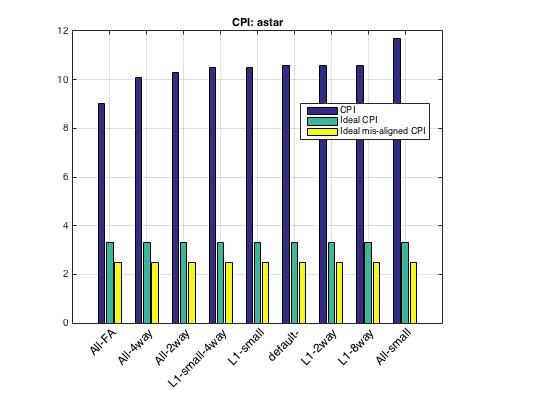
\includegraphics[scale=0.75]{CPIastar}
            \caption{astar CPI}
            \label{fig:CPIastar}
        \end{figure}

    \subsection{bzip2}
        \begin{figure}[H]
            \centering
            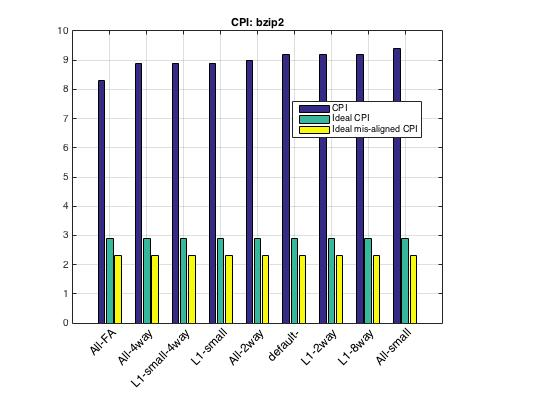
\includegraphics[scale=0.75]{CPIbzip2}
            \caption{bzip2 CPI}
            \label{fig:CPIbzip2}
        \end{figure}

    \subsection{gobmk}
        \begin{figure}[H]
            \centering
            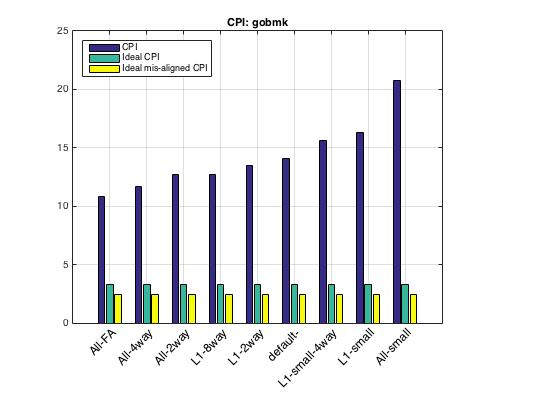
\includegraphics[scale=0.75]{CPIgobmk}
            \caption{gobmk CPI}
            \label{fig:CPIgobmk}
        \end{figure}

    \subsection{libquantum}
        \begin{figure}[H]
            \centering
            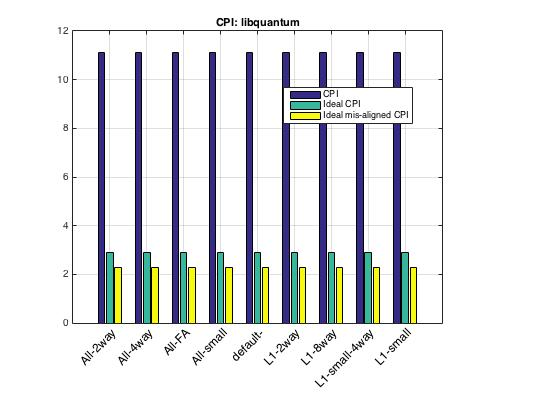
\includegraphics[scale=0.75]{CPIlibquantum}
            \caption{libquantum CPI}
            \label{fig:CPIlibquantum}
        \end{figure}

    \subsection{omnetpp}
        \begin{figure}[H]
            \centering
            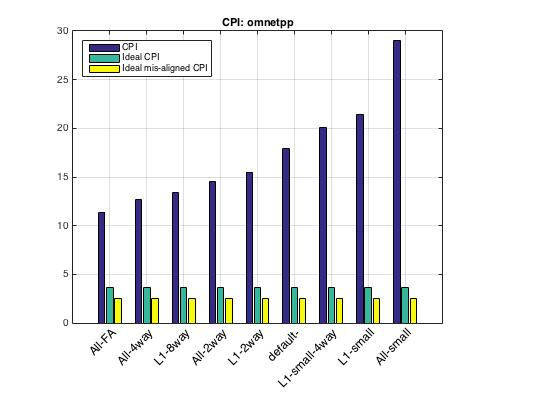
\includegraphics[scale=0.75]{CPIomnetpp}
            \caption{omnetpp CPI}
            \label{fig:CPIomnetpp}
        \end{figure}

    \subsection{sjeng}
        \begin{figure}[H]
            \centering
            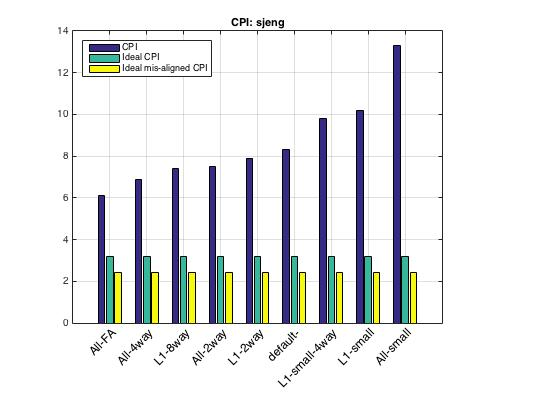
\includegraphics[scale=0.75]{CPIsjeng}
            \caption{sjeng CPI}
            \label{fig:CPIsjeng}
        \end{figure}

\section{Overall Performance Comparison}
\begin{figure}[H]
            \centering
            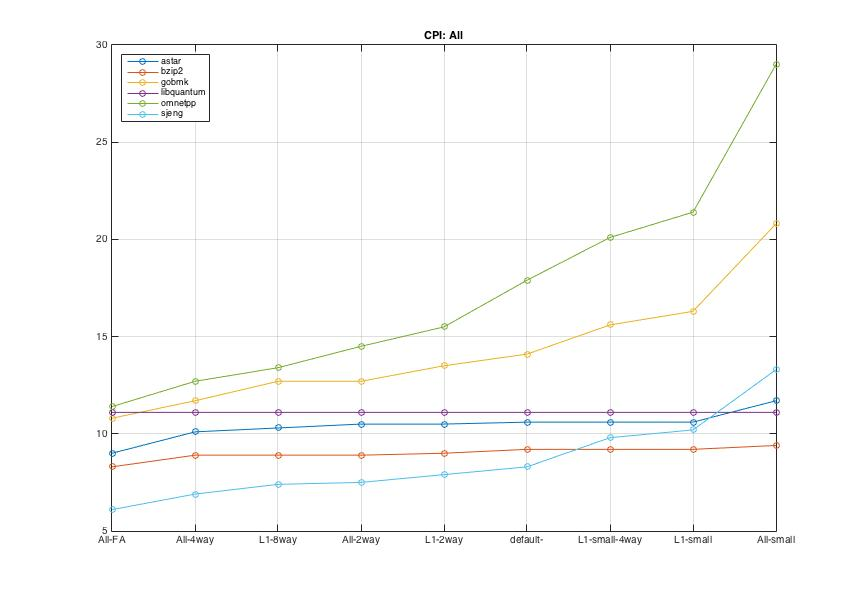
\includegraphics[scale=0.5]{CPIall}
            \caption{CPI comparison}
            \label{fig:CPIall}
        \end{figure}
        
\section{Cost Evaluation}
    An additional method used to evaluate the different cache configurations is to look at the cost associated with a particular configuration. The costs are evaluated based on the following information:
    \begin{itemize}
        \item L1 cache
            \begin{itemize}
                \item \$100 for each 4KB
                \item \$100 for each doubling in associativity beyond direct-mapped
            \end{itemize}
        \item L2 cache
            \begin{itemize}
                \item \$50 per 16KB
                \item \$50 for each doubling in associativity beyond direct-mapped
            \end{itemize}
        \item Main memory
            \begin{itemize}
                \item base latency of 50 costs \$50
                \item base 8-byte mem chunk-size bandwidth costs \$25
                \item \$100 to increase the bandwidth (mem chunk-size) by a factor of 2
            \end{itemize}
    \end{itemize}

    \subsection{Cost by configuration}
        Figure \ref{fig:totCost} shows the breakdown of the memory cost for each of the different configurations. The overall cost is shown as well as the cost for each level in the memory hierarchy. This plot shows that the All-small configuration results in the lowest cost while the All-FA (fully associative) configuration results in the highest cost. Section \ref{sec:costVperf} examines the relation between cost and performance.
        \begin{figure}[H]
            \centering
            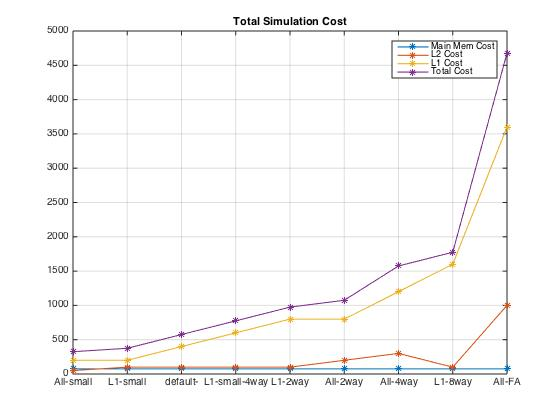
\includegraphics[scale=0.75]{totalCost}
            \caption{Cost by configuration}
            \label{fig:totCost}
        \end{figure}

    \subsection{Cost versus Performance} \label{sec:costVperf}
        The following series of bar graphs displays the CPI versus cost for each trace and configuration. The values for the cost are divided by 100 and then the data is normalized between 0-1. This was necessary in order to display the large values of cost with the relatively lower values of CPI. Each plot is sorted with the best performance (shown in yellow) on the left. The cost associated with that performance level is represented in blue next to the CPI value. Clearly, the best performance is given by the fully associative configuration but this option also results in the highest cost. A better choice would be to use these plots and select the lowest CPI with the correspondingly lowest cost. The best option is somewhat subjective and related to the budget available when designing the cache but the All-2way configuration provides a decently low CPI while still maintaining a low cost.
        \begin{figure}[H]
            \centering
            \begin{minipage}{.5\textwidth}
                \centering
                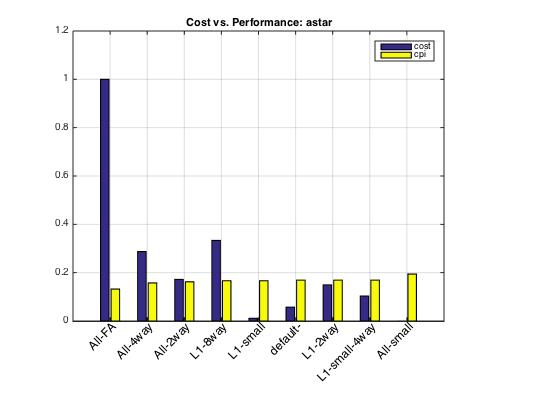
\includegraphics[width=10cm]{cvpastar}
                \caption{Cost vs. CPI astar}
                \label{fig:cvpastar}
            \end{minipage}%
            \begin{minipage}{.5\textwidth}
                \centering
                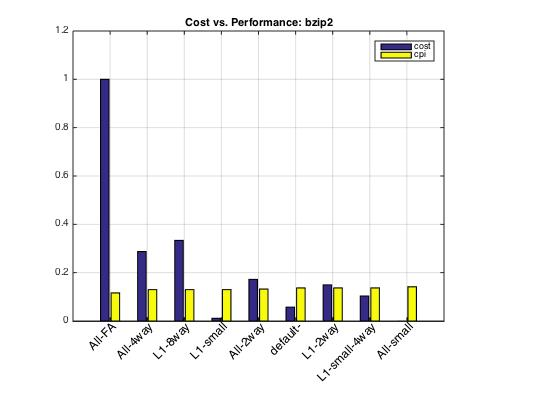
\includegraphics[width=10cm]{cvpbzip2}
                \caption{Cost vs. CPI bzip2}
                \label{fig:cvpbzip2}
            \end{minipage}
        \end{figure}
        \begin{figure}[H]
            \centering
            \begin{minipage}{.5\textwidth}
                \centering
                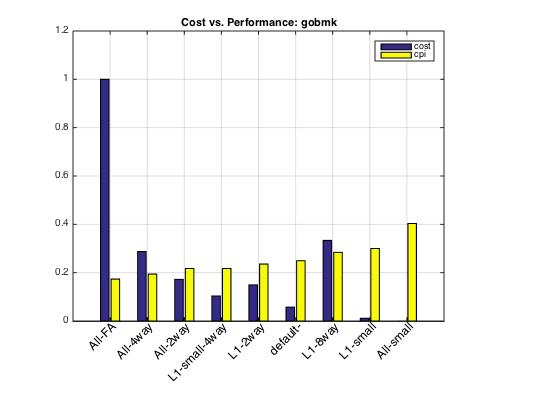
\includegraphics[width=10cm]{cvpgobmk}
                \caption{Cost vs. CPI gobmk}
                \label{fig:cvpgobmk}
            \end{minipage}%
            \begin{minipage}{.5\textwidth}
                \centering
                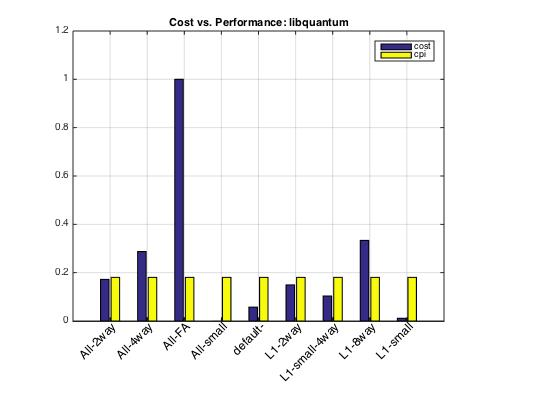
\includegraphics[width=10cm]{cvplibquantum}
                \caption{Cost vs. CPI libquantum}
                \label{fig:cvplibquantum}
            \end{minipage}
        \end{figure}
        \begin{figure}[H]
            \centering
            \begin{minipage}{.5\textwidth}
                \centering
                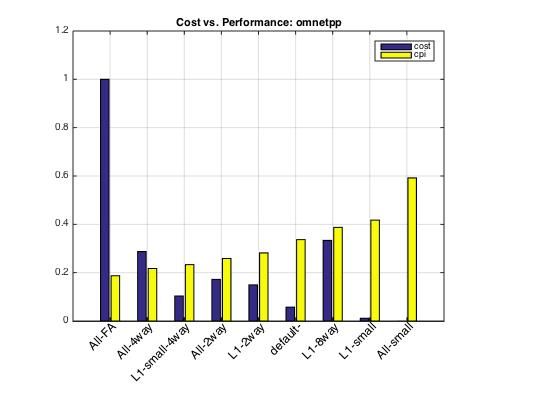
\includegraphics[width=10cm]{cvpomnetpp}
                \caption{Cost vs. CPI omnetpp}
                \label{fig:cvomnetpp}
            \end{minipage}%
            \begin{minipage}{.5\textwidth}
                \centering
                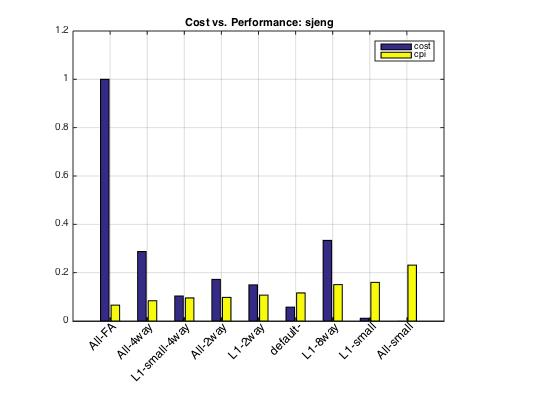
\includegraphics[width=10cm]{cvpsjeng}
                \caption{Cost vs. CPI sjeng}
                \label{fig:cvpsjeng}
            \end{minipage}
        \end{figure}

\section{Main Memory Bandwidth Increase}
   A method that can be used to increase the memory system performance is to increase the bandwidth to main memory. The base configuration uses a mem chunk-size of 8 bytes. Increasing this value will speed up each access to main memory. To evaluate the performance gains when the bandwidth is increased we ran three additional simulations using the sjeng trace. Each additional simulation used the default configuration with the bandwidth to main memory increasing from the default 8 bytes to 16, 32, and 64 bytes. The increase in bandwidth results in an associated increase in cost of \$100 for each doubling of mem chunk-size. Figure \ref{fig:exSj} displays the CPI versus cost using the same method described in section \ref{sec:costVperf}. It can be seen that the increasing the bandwidth to 64 bytes results in the lowest CPI of 6.3 but the cost is the highest. The base cost with a bandwidth of 8 bytes if \$575 and increasing the bandwidth to 64 bytes results in a cost of \$875. The cost increase of \$300 is fairly low and the CPI is reduced from 8.3 to 6.3. Our analysis it that accepting the additional cost to increase the bandwidth to 64 bytes is an acceptable compromise to realize a 25\% decrease in CPI.
   \begin{figure}[H]
       \centering
       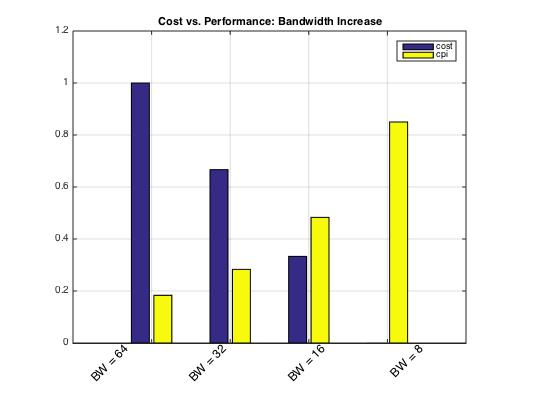
\includegraphics[scale=0.75]{extraSjeng}
       \caption{Cost vs. Performance: Bandwidth Increase}
       \label{fig:exSj}
   \end{figure}

\section{Conclusion}

\end{document}
